\chapter{Memory management framework for derivative clouds}
 
  \section{Drawbacks of existing framework}
  
    \subsection{Provisioning of caches at different levels based on application requirements}
      
  
    \subsection{Inability of cache partitioning framework to support anonymous memory applications}    
    

  \section{Rethink of existing design}
  
    \subsection{Decentralized memory management framework}
	      
      \subsubsection{Native provider cache partitioning framework}

      \subsubsection{Derivative provider memory management framework}	

    \subsection{Hybrid cache}
      
      \subsubsection{Multilevel configurable caches}
      
      \subsubsection{Movement of cache objects}
	
  \newpage
  
  \section{Implementation details}
      
    \subsection{Existing implementation status}
    
    \subsection{Hybrid cache}
    
      \subsubsection{Pools to accommodate both memory and SSD objects}
      
      \subsubsection{Asynchronous kernel threads for movement of objects}
      
      \subsubsection{Multilevel stats}
  
  \newpage
  
  \section{Correctness of implementation}
  
    \subsection{Experimental setup}
	
      The following section describes the experimental setup used to verify the correctness of our implementation. 
	
      \myparagraph{Experimental configurations}	
	The set of configurations used for an analysis of memory management framework for a derivative environment 
	must be relevant, and easy to apply. The following configurations
fit this criteria, and have been used for the evaluation.

	  \begin{itemize}
	   \item \textbf{Memory Requirement:} Memory requirement of each container, the estimated total memory used by a container.
	   
	   \item \textbf{Container memory limit:} Size of memory allocated to a container at the Cgroup level (soft and hard limits). 
	   \item \textbf{Memory cache limit:} Size of memory (L1) cache assigned to a container. 
	   \item \textbf{SSD cache limit:} Size of SSD (L2) cache assigned to a container.
	   
	   \item \textbf{Workload:} Workload application that is running inside each of the container. 
	   \item \textbf{Number of containers:} Number of containers that are currently executing in the system.
	   \item \textbf{Number of VMs:} Number of virtual machines that are currently executing in the system.
	  \end{itemize}	  
	  
	  For the sake of simplicity in the evaluations of correctness of our setup. We have only considered a single container, single VM setup 
	  which makes use of synthetic workload to stress our system.
	
      \myparagraph{Metrics of interest}	
	The following are the metrics of interest that would help us establish the correctness of our implementation.
	  
	  \begin{itemize}
	   
	   \item \textbf{Container memory usage:} Guest memory usage of the container.
	   \item \textbf{Memory cache usage:} Memory cache used by the container.
	   \item \textbf{SSD cache usage:} SSD cache used by the container.
	   
	   \item \textbf{Demoted:} Objects moved from memory to SSD cache.
	   \item \textbf{Promoted:} Objects moved from SSD to memory cache.
	   
	  \end{itemize}	  
	  
	  The following metrics are collected both for memory and SSD cache
	  
	  \begin{itemize}
	   
	   \item \textbf{Puts:} Number of objects successfully put into this container cache.
	   \item \textbf{Gets:} Number of objects successfully got from this container cache.
	   \item \textbf{Flushes:} Number of objects flushed from this container cache.
	   \item \textbf{Evicts:} Number of objects evicted from this container cache.
	   
	  \end{itemize}	  
	  
	
      \myparagraph{Workload}
      \label{section:correctness_workload}
	For establishing the correctness of our workload, we have considered a self generated workload generated using \texttt{cat} command 
	that outputs the content of a file onto \texttt{/dev/null}.
	
      \myparagraph{Testbed}	
	Our testbed consists of a single VM, single container running on top of our hybrid implementation of Double decker as shown 
	in Fig~\ref{img:correctness_testbed}. The hypervisor used is KVM, and the container manager used is LXC.  
	
	
	\noindent The physical machine configuration used is as described below,
	  \begin{enumerate}
	   \item Intel(R) Core(TM) i7-3770 CPU @ 3.40GHz
	   \item 4 CPU cores (with multi-threading)
	   \item 8 GB of physical RAM
	   \item 120 GB SSD disk
	  \end{enumerate}

	
	\begin{figure}
	  \centering
	  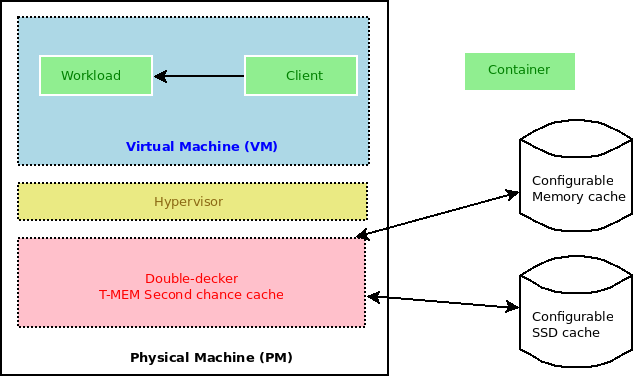
\includegraphics[width=0.9\textwidth]{images/correctness/exp_setup.png}
	  \caption{Experimental testbed for checking correctness}
	  \label{img:correctness_testbed}
	\end{figure}
  
    \subsection{Arithematic validation of stats}
    
      \myparagraph{Question}
	    To verify the correctness in accounting of stats while accessing cache at both levels.
	    
      \myparagraph{Procedure}
	We ran several experiments and computed the actual cache usage (memory and SSD) in our implementation. To an calculated 
	an estimated cache usage we used the formula given below. We used the same formula for both memory and SSD cache. 
	  \begin{equation}
	    EstimatedUsed = Puts + ObjectsMovedIn - (Gets + Flushes + ObjectsMovedOut)
	  \end{equation}
      
      \myparagraph{Observations}
	The values for \textit{EstimatedUsed} and \textit{ActualUsed} (present in out stat counter) matched in most cases.
	However, over long periods of run, with quite a large number of cache operations there was a marginal difference
	between the two (\textless 1\%).
	
      \myparagraph{Inference}
	Since the correctness of the actual value of cache used depend on the other stats that we have collected, and the 
	matching of \textit{EstimatedUsed} and \textit{ActualUsed} would only mean that all the stats collected are right.
    
    \subsection{Movement of objects between both levels of cache}
	
	To verify the correctness of our implementation empirically, we have taken our synthetic workload described in 
	section~\ref{section:correctness_workload} and ran a couple of simple experiments to demonstrate the expected 
	behavior of our cache to support cache operations like puts, gets, promotions and demotions.  
	
	\subsubsection{Memory to SSD cache}

	  \myparagraph{Question}
	    To verify the correctness in accounting of stats while accessing cache and moving objects from memory (L1) to SSD (L2) cache.
	    
	  \myparagraph{Procedure}
	      We start of the experiment with powering on the VM, followed by the container. We assigned complete memory and SSD cache 
	    at the double-decker back-end to support the container. The container had a \textbf{memory requirement of 2078 MB}, 2048 MB workload
	    requirement and 30 MB container requirement (container requirement was obtained by running the same experiment while having
	    a nearly 0 MB workload. The container was allocated with 2048 MB (512 MB of container memory + 512 MB of memory cache 
	    + 1024 MB of SSD cache). Now, the workload performed a sequential read of its workload (i.e 2048 MB) once.
	    Table~\ref{table:correctness_memtossd} shows the list of approx. estimated values (which are based on our 
	    implementation) and observed values for the metrics at the cache at the end of the experiment. 
	    
	    \vspace*{1em}	
	      \begin{table}
		\begin{center}
		  \begin{tabular}{ r | p{4cm} | p{4cm} }	      	    
			Metric & Approx. estimated Value & Observed Value \\ 
		    \hline
		    \hline
		    Puts (MB) & 2078 & 2080 \\
		    \hline
		    Gets (MB) & 0 & 1 \\
		    \hline
		    Container memory usage (MB) & 512 & 509 \\  
		    \hline
		    Memory cache usage (MB) & 504 & 503 \\
		    \hline 
		    SSD cache usage (MB) & 1008 & 1000 \\
		    \hline
		    Evicts (MB) & 54  & 64 \\
		    \hline
		    Flushes (MB) & 0  & 0 \\
		    \hline
		    Cumulative usage (MB) & 2078 & 2076 \\
		    \hline
		    Demotions (MB) & 1062 & 1064 \\
		    \hline
		    
		  \end{tabular}
		\caption{Comparison between expected and actual values}
		\label{table:correctness_memtossd}
		\end{center}	  
	      \end{table}
	    \vspace*{1em}
	    
	  \myparagraph{Observations}
	  The following are the observations,	  
	    \begin{enumerate}
	     \item There is a small number of gets, probably occurring due to pages used by other container applications.
	     \item Puts in the cache, is marginally (\textless2 MB) greater than expected value, and this deviation is due to the small number 
	     of Gets which are occurring.
	     \item The memory cache usage, is exactly as expected. However, SSD cache usage is slightly lesser than the expected value, 
	     but however the deviation seems to be an acceptable value.
	     \item The demotions (movement from memory to SSD) and cumulative usage values are nearly the same with a subtle deviation 
	     (\textless2 MB) which is an acceptable value.
	    \end{enumerate}

	  
	  \myparagraph{Inference}
	    The accounting stats, are nearly as expected. This verifies the correctness of most of the stats of our implementation (except promotions).
	    
	
	\subsubsection{SSD to memory cache}
	  
	  \myparagraph{Question}
	    To verify the correctness in accounting of stats while moving objects from SSD (L2) to memory (L1) cache.
	    
	  \myparagraph{Procedure}
	      We start of the experiment with powering on the VM, followed by the container. We assigned complete memory and SSD cache 
	    at the double-decker back-end to support the container. The container had a \textbf{memory requirement of 2078 MB}, 2048 MB workload
	    requirement and 30 MB container requirement (container requirement was obtained by running the same experiment while having
	    a nearly 0 MB workload. The container was allocated with 2560 MB (512 MB of container memory + 2048 MB of SSD cache).
	    The workload performed a sequential read of its workload (i.e 2048 MB) once, this lead to using up of nearly 1566 MB of SSD cache.
	    
	    Now, we changed the memory cache size to 256 MB while performing basic operations at the container which triggered the promotion 
	    (movement of objects from SSD to memory) of the objects to the memory cache. The promotion triggers all objects until the memory 
	    cache reaches a threshold usage - 192 MB in our case, as this threshold is calculated as,
	    
	    \begin{equation}
	      MemoryCacheLowerThreshold (192 MB) = MemoryLimit (256 MB) - LimitSize (64 MB)
	    \end{equation}
	    
	    Hence we would expect 192 MB worth of objects be promoted from SSD to memory cache in an ideal case.
	    
	    
	  \myparagraph{Observation}
	    Using our stats, it was observed that the estimated promotion and the actual promotion of objects were of an exact match with 
	    the number being 192 MB.
	    
	  \myparagraph{Inference}
	    This verifies the correctness in the accounting stats in movement of objects from SSD to memory cache. Hence movement 
	    of objects from both memory to SSD and vice-versa have been verified empirically.
  
  
  
  \section{Evaluation of Double Decker}
  
    \subsection{Experimental setup}
	
	\paragraph{Experimental configurations}
	
	\paragraph{Metrics of interest}
	
	\paragraph{Workload}
	
	\paragraph{Testbed}
  
    %\subsection{Performance comparion with old implementation}
  
    \subsection{Provisioning for anonymous and file backed workloads}
    
    \subsection{Hybrid cache provisioning}
    